\documentclass[11pt]{article}
\usepackage{paper_style}

\usepackage{graphicx} % Required for inserting images
\usepackage{indentfirst}
\usepackage{lipsum}
\usepackage{array}
\usepackage{float}
\usepackage{longtable}
\usepackage{enumitem}
\usepackage{hyperref}
\usepackage{float}

%% ===============================================
%% Setting the line spacing (3 options: only pick one)
% \doublespacing
% \singlespacing
\onehalfspacing
%% ===============================================

\setlength{\droptitle}{-5em} %% Don't touch

\title{Investigation of the Relationship between Temperature and Resistance of a Thermistor}
\author{Saptak Das}
\date{April 2023}

\begin{document}

\maketitle

\section{Introduction}
\label{section:introduction}
I have always had a passion for electronics engineering, specifically how electronic sensors act as an interface for a computer to understand and interact with the complex environment it exists in. Specifically, I wondered how refrigerators, ovens, and HVAC knew when to turn on and turn off. I knew that thermistors were at the core of all these devices, but I could not determine how they functioned. Hence, I decided to explore how temperature affects the resistance of a thermistor for my Physics Internal Assessment.

Furthermore, I have always been curious about the workings of superconductors, their unique properties, and their widespread applications. However, most superconductors must be cooled down significantly (around 93 K) before they exhibit their characteristic “zero resistance” \citep{butera1997dependence}. This experiment was thus currently infeasible, however, this investigation of the relationship between temperature and resistance in thermistors could be an important stepping stone for an experiment examining this same relationship in superconductors.

\subsection{Research Question}
What is the relationship between the electrical resistance and the temperature of a negative temperature coefficient (NTC) thermistor? 

\section{Background Research}
\subsection{Temperature Coefficient of Resistance}
The temperature coefficient of resistance (TCR) is a measure of how much the resistance of a material changes with temperature. 

\[TCR = \frac{R-R_0}{R_0(T-T_0)}\]

TCR is defined as the change in resistance per unit change in temperature, usually expressed in parts per million per degree Celsius (ppm/°C) or per Kelvin (ppm/K) \citep{feteira2009negative}.  If the TCR of a material is positive, the material's resistance increases with temperature. If the TCR is negative, then the material's resistance decreases with temperature.

\begin{figure}[H]
    \centering
    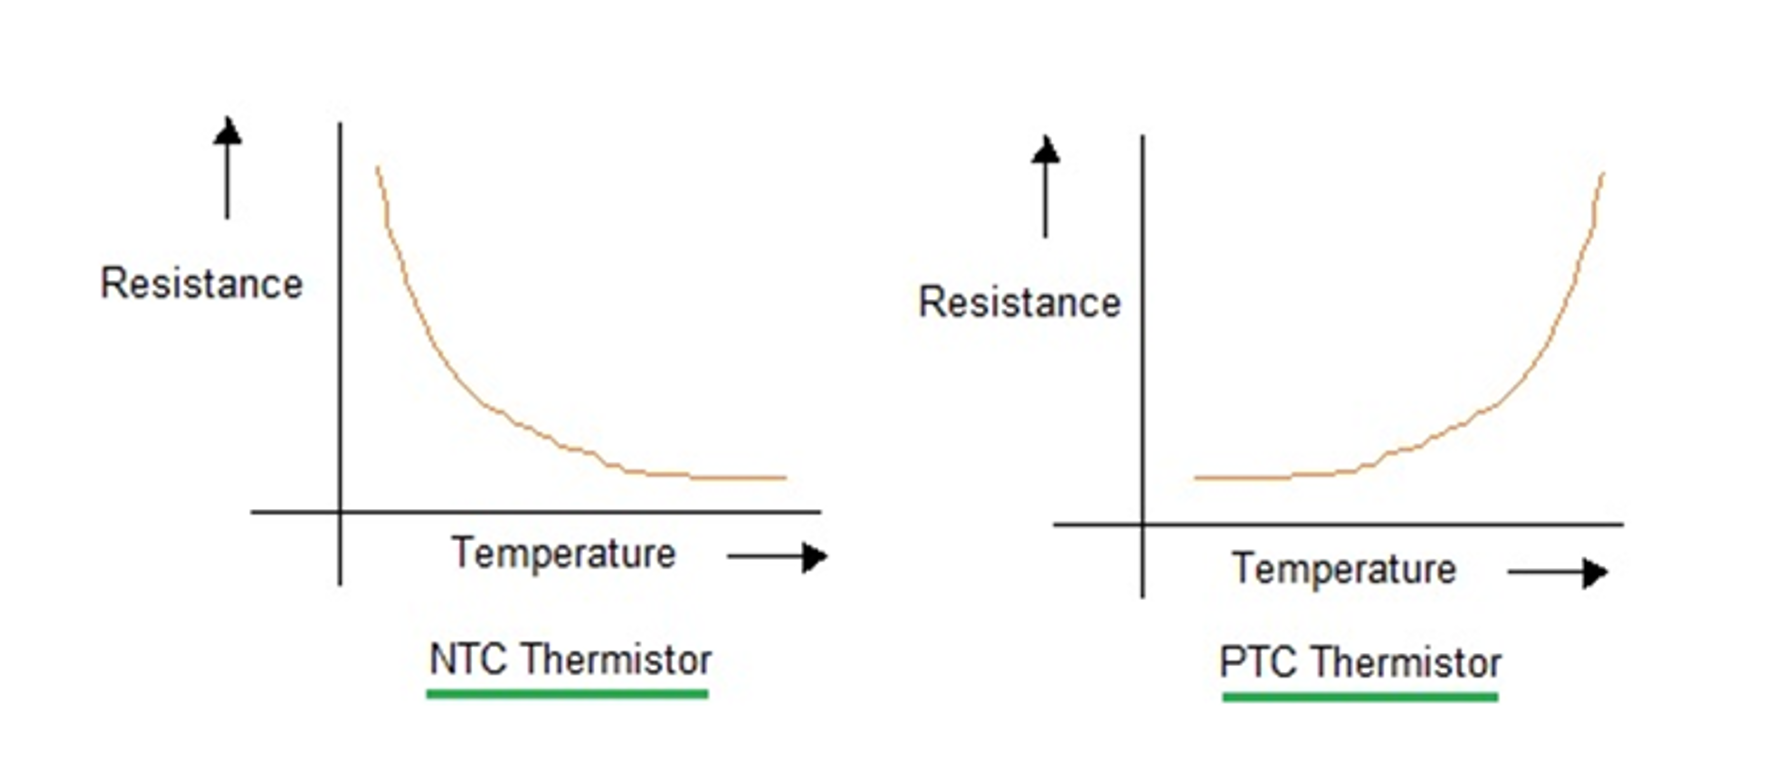
\includegraphics[width=130mm,height=\textheight,keepaspectratio]{images/ntc_ptc.png}
    \caption{Resistance vs Temperature Graph for NTC and PTC Thermistors \citep{amethermptcntc}}
    \label{fig:ntc_ptc}
\end{figure}

\subsection{Conductor - Resistance vs Temperature}
Temperature has a significant effect on the resistance of a regular conductive metallic substance. As the temperature of a metal increases, its resistance also increases. This positive TCR is due to the fact that the increased temperature causes the electrons in the metal to vibrate more and thus collide with each other more often, increasing the resistance \citep{butera1997dependence}. The magnitude of the temperature coefficient of resistance varies from one metal to another, with some metals having a higher coefficient than others.

\subsection{Semiconductor - Resistance vs Temperature}
Temperature impacts the resistance of a semiconductor in two ways. First, as temperature increases, the mobility of the charge carriers in the semiconductor increases, which reduces the resistance of the semiconductor. Second, as temperature increases, more charge carriers are generated, which also reduces the resistance of the semiconductor \citep{butera1997dependence}. Thus, at low temperatures close to absolute zero, the resistance of a semiconductor is very high. The temperature coefficient of resistance (TCR) of a semiconductor is usually negative, meaning that resistance decreases with increasing temperature. The TCR of a semiconductor is dependent on the type of semiconductor material and the doping level.

\begin{figure}[H]
    \centering
    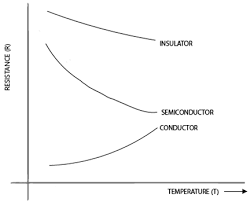
\includegraphics[width=75mm,height=\textheight,keepaspectratio]{images/conductor_semiconductor_insulator.png}
    \caption{Resistivity vs Temperature Graph for Conductors, Semiconductors, and Insulators \citep{mandal_2022}. This plot shows the positive TCR of conductors and the negative TCR for semiconductors and insulators.}
    \label{fig:materials_RT_Plot}
\end{figure}

\section{Hypothesis}
If the temperature of an NTC thermistor increases, then the resistance of the NTC thermistor will decrease exponentially. If the temperature of an NTC thermistor decreases, then the resistance of the NTC thermistor will increase exponentially. 

\section{Variables}
\subsection{Independent Variables and Dependent Variables}
The independent variable for this experiment is the temperature of the NTC Thermistor, which is measured by a Vernier Temperature Probe with a precision of $\pm 0.1^\circ C$. The dependent variable for my experiment is the electrical resistance of the NTC Thermistor, which is measured using a Multimeter configured as an Ohmmeter with a precision of $\pm 0.01 \; k\Omega$.

Since all data is being collected after running all trials, the high precision of video analysis can be utilized, which greatly increases both the accuracy and precision of the resistance and temperature data. More details about the specific measurement processes are described in the Section \ref{section:procedure} \nameref{section:procedure}.

\subsection{Control Variables}
I ensured that all other variables were controlled to get accurate results about the relationship between the resistance and temperature. For example, throughout the trials, the circuit remained untouched so that no variations would occur due to the connections. Furthermore, the same amount of water ($150 \; mL$) at roughly the same initial temperature ($<20^\circ C$) was used for every trial with the same heating source to ensure that the controlled temperature increased at the same rate throughout the trials. Finally, the beaker, temperature probe, and thermistor were always cooled down to room temperature before proceeding to do a new trial. Through all measures, a more accurate relationship between my independent and dependent variables can be assessed.

\section{Methodology}
\subsection{Materials}
\begin{itemize}[noitemsep]
    \item NTC Thermistor (E305314; HXT-600; Max Operating Temperature: $105^\circ C$)
    \item Vernier Temperature Probe, $\pm 0.1^\circ C$
    \item GoLink (for connecting to Logger Pro)
    \item Logger Pro Software on Laptop (for dynamic temperature logging)
    \item Multimeter (as use as Ohmmeter), $\pm 0.01 \; k\Omega$ 
    \item Heat Source (Gas Stovetop used in this experiment, though Bunsen Burner or Heating Plate could be used)
    \item Phone and Tripod Stand (to record experiment)
    \item $400 \; mL$ Glass Beaker
    \item Beaker Tongs and Wire Gauze (to move hot beaker and evenly heat up and cool down beakers respectively)
    \item $150 \; mL$ of Water initially at $<20^\circ C$ (medium to heat up thermistor)
\end{itemize}

\subsection{Experimental Setup}
\begin{figure}[ht]
    \centering
    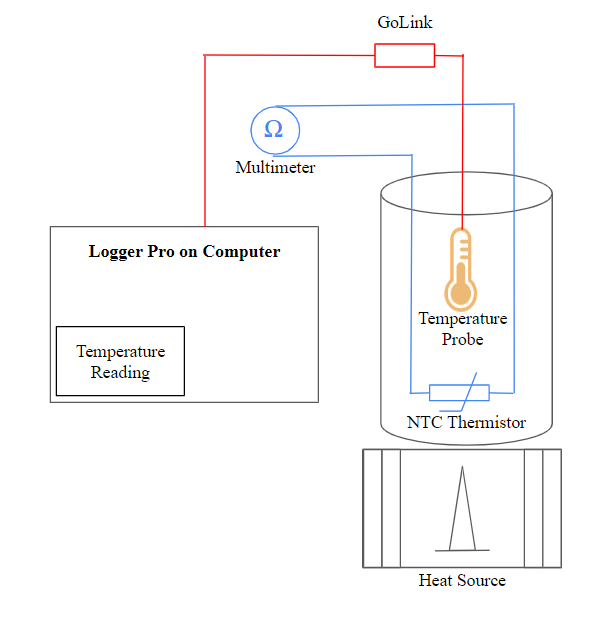
\includegraphics[width=\textwidth,height=100mm,keepaspectratio]{images/IA_Schematic.png}
    \caption{Schematic for Physics IA Experiment Setup}
    \label{fig:schematic}
\end{figure}


\begin{figure}[ht]
    \centering
    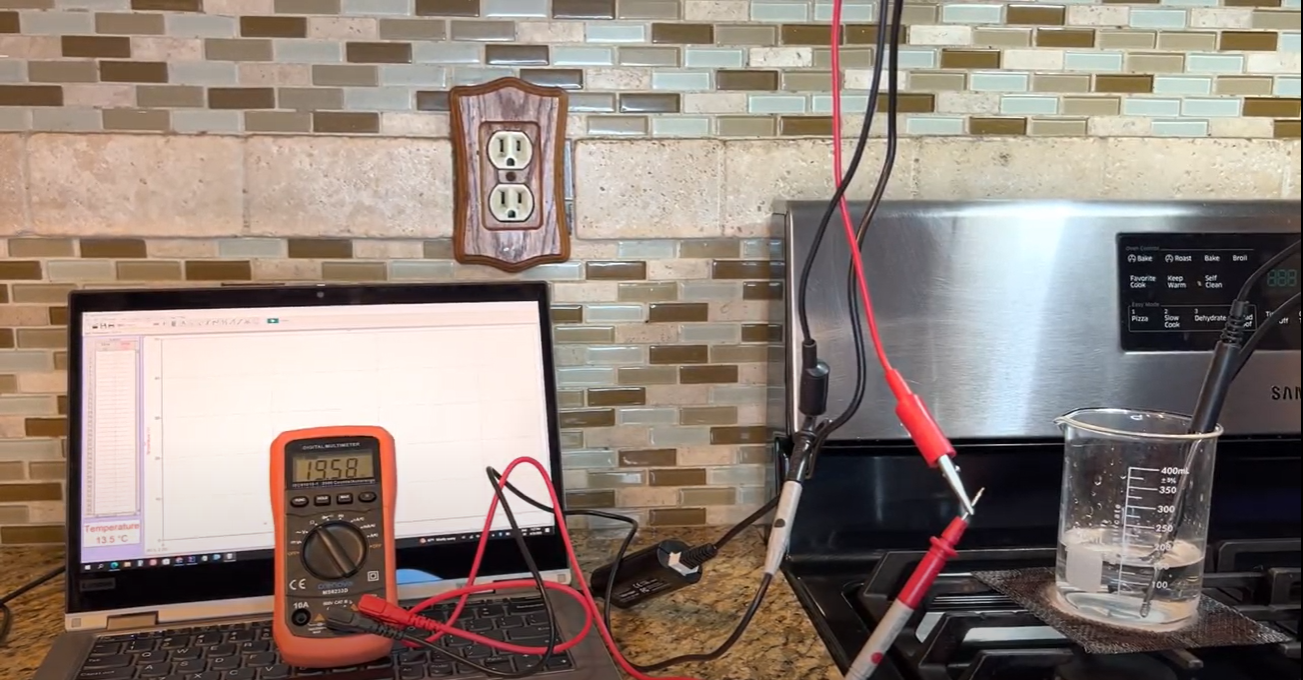
\includegraphics[width=120mm,height=\textheight,keepaspectratio]{images/setup.png}
    \caption{Example Image of Phone Footage at Start of Experiment}
    \label{fig:footage}
\end{figure}

\section{Procedure}
\label{section:procedure}
\begin{enumerate}[noitemsep]
    \item Put Multimeter in Ohmmeter mode and attach each of the leads to the thermistor leads. Plug Vernier Temperature Probe into the laptop via the GoLink. Open up Logger Pro software to get live temperature reading. Place Wire Gauze on Gas Stovetop. Setup the Tripod Stand with Phone such that the Multimeter and Temperature Probe readings are clearly visible.
    \item Now, for each of the 5 trials:
    \begin{enumerate}[noitemsep]
        \item Fill the Glass Beaker with $150 \; mL$ of water, which is initially below $20^\circ C$, and place it on the Wire Gauze. Put the Temperature Probe and the NTC Thermistor near the center of the beaker.
        \item Start recording the trial using the phone-tripod setup. Put the heat at the lowest setting so that the temperature rises slowly and evenly.
        \item once the water starts boiling at $~100^\circ C$, end the recording and turn off the heating from the stove. Remove the Temperature Probe and NTC Thermistor from the Beaker. Use the Beaker Tongs to carry the hot beaker and dump out the boiling water. Leave the Glass Beaker on the Wire Gauze to cool back down to room temperature.
    \end{enumerate}
    \item Using all the footage collected in the previous step, the 16 levels of resistance and temperature data points must be collected. For each video:
    \begin{enumerate}[noitemsep]
        \item Slowly scroll through the video till you get to exactly $20.0^\circ C$. Record the resistance reading at this temperature in a table.
        \item Repeat this process in $5^\circ C$ increments until $95^\circ C$ is reached. 
    \end{enumerate}
\end{enumerate}

\section{Safety and Ethics}
Throughout this investigation, all safety and ethical concerns were recognized and thoroughly addressed. The main hazard in this lab is the heating source. Thus, multiple solutions were implemented to mitigate risks. First, the experiment was approved and performed under teacher supervision. Second, proper experiment apparatus such as wire gauze and beaker tongs were used. Finally, the glass beaker was cooled slowly to ensure that it would not shatter upon a rapid temperature change. All these measures greatly improved safety, leading to no injuries during the course of the experiment.

\section{Data Collection}
\subsection{Quantitative Raw Data}

\begin{longtable}{|c|c|c|c|c|c|}
    \hline
    Temperature (± 0.1 °C) & \multicolumn{5}{| c |}{Resistance (± 0.01 $k\Omega$)} \\ \hline
    ~ & Trial 1 & Trial 2 & Trial 3 & Trial 4 & Trial 5 \\ \hline
    20.0 & 20.00 & 14.40 & 16.60 & 17.03 & 17.58 \\ \hline
    25.0 & 16.05 & 11.93 & 13.88 & 14.07 & 14.40 \\ \hline
    30.0 & 13.88 & 10.15 & 12.14 & 11.46 & 12.37 \\ \hline
    35.0 & 11.54 & 8.88 & 10.16 & 9.71 & 10.36 \\ \hline
    40.0 & 9.51 & 7.65 & 8.83 & 8.28 & 8.70 \\ \hline
    45.0 & 8.07 & 6.47 & 7.61 & 6.89 & 7.34 \\ \hline
    50.0 & 6.89 & 5.98 & 6.39 & 5.89 & 6.19 \\ \hline
    55.0 & 5.39 & 4.62 & 5.33 & 5.01 & 5.30 \\ \hline
    60.0 & 4.42 & 3.88 & 4.69 & 4.30 & 4.56 \\ \hline
    65.0 & 3.83 & 3.40 & 3.84 & 3.68 & 3.82 \\ \hline
    70.0 & 3.25 & 2.91 & 3.28 & 3.11 & 3.27 \\ \hline
    75.0 & 2.73 & 2.41 & 2.69 & 2.62 & 2.79 \\ \hline
    80.0 & 2.37 & 2.10 & 2.29 & 2.25 & 2.33 \\ \hline
    85.0 & 1.98 & 1.81 & 1.94 & 1.92 & 1.98 \\ \hline
    90.0 & 1.74 & 1.57 & 1.69 & 1.66 & 1.70 \\ \hline
    95.0 & 1.51 & 1.48 & 1.53 & 1.45 & 1.49 \\ \hline
\caption{Resistance of an NTC Thermistor at a given Temperature}
\end{longtable}

\subsection{Qualitative Observations}
\begin{itemize}[noitemsep]
    \item With the heating on the lowest setting, the temperature incremented evenly at a rate of approximately $1^\circ C$ every 2-3 seconds.
    \item The trials seem to affirm that the resistance decreases as the temperature increases, which is indicative of the negative TCR of NTC Thermistors.
    \item At the beginning of Trial 1 and Trial 2, I noticed that the resistance differed by almost $6 \; k\Omega$ for roughly the same temperature ($20.0^\circ C$).
    \item The pattern mentioned above continued throughout the various other trials, though the effect was less pronounced.
\end{itemize}


\section{Analysis}
\subsection{Processed Data}
In order to derive the relationship in the data, I first determined the average resistance. To calculate the absolute and percent average uncertainty for the resistances, the following formulas can be applied. Sample calculations for $T=20^\circ C$ are shown below.
\[\delta R_{avg}=\frac{R_{max}-R_{min}}{2\sqrt{N}}=\frac{20.00\;k\Omega -14.40\;k\Omega}{2\sqrt{5}}=1.25\;k\Omega\]

\[\frac{\delta R_{avg}}{R_{avg}}=\frac{1.25\;k\Omega}{17.12\;k\Omega}=7.31\%\]

\begin{longtable}{| >{\centering\arraybackslash}p{0.17\linewidth} | >{\centering\arraybackslash}p{0.15\linewidth} | >{\centering\arraybackslash}p{0.25\linewidth} | >{\centering\arraybackslash}p{0.25\linewidth} |}
\hline
    Temperature (± 0.1 °C) & Average Resistance ($k\Omega$) & Average Resistance Uncertainty ($k\Omega$) & Average Resistance Uncertainty (\%) \\ \hline
    20.0 & 17.12 & 1.25 & 7.31 \\ \hline
    25.0 & 14.07 & 0.92 & 6.55 \\ \hline
    30.0 & 12.00 & 0.83 & 6.95 \\ \hline
    35.0 & 10.13 & 0.59 & 5.87 \\ \hline
    40.0 & 8.59 & 0.42 & 4.84 \\ \hline
    45.0 & 7.28 & 0.36 & 4.92 \\ \hline
    50.0 & 6.27 & 0.22 & 3.57 \\ \hline
    55.0 & 5.13 & 0.17 & 3.36 \\ \hline
    60.0 & 4.37 & 0.18 & 4.14 \\ \hline
    65.0 & 3.71 & 0.10 & 2.65 \\ \hline
    70.0 & 3.16 & 0.08 & 2.61 \\ \hline
    75.0 & 2.65 & 0.08 & 3.21 \\ \hline
    80.0 & 2.27 & 0.06 & 2.66 \\ \hline
    85.0 & 1.93 & 0.04 & 1.96 \\ \hline
    90.0 & 1.67 & 0.04 & 2.26 \\ \hline
    95.0 & 1.49 & 0.02 & 1.20 \\ \hline
\caption{Average Resistance of an NTC Thermistor at a given Temperature}
\end{longtable}

\begin{figure}[H]
    \centering
    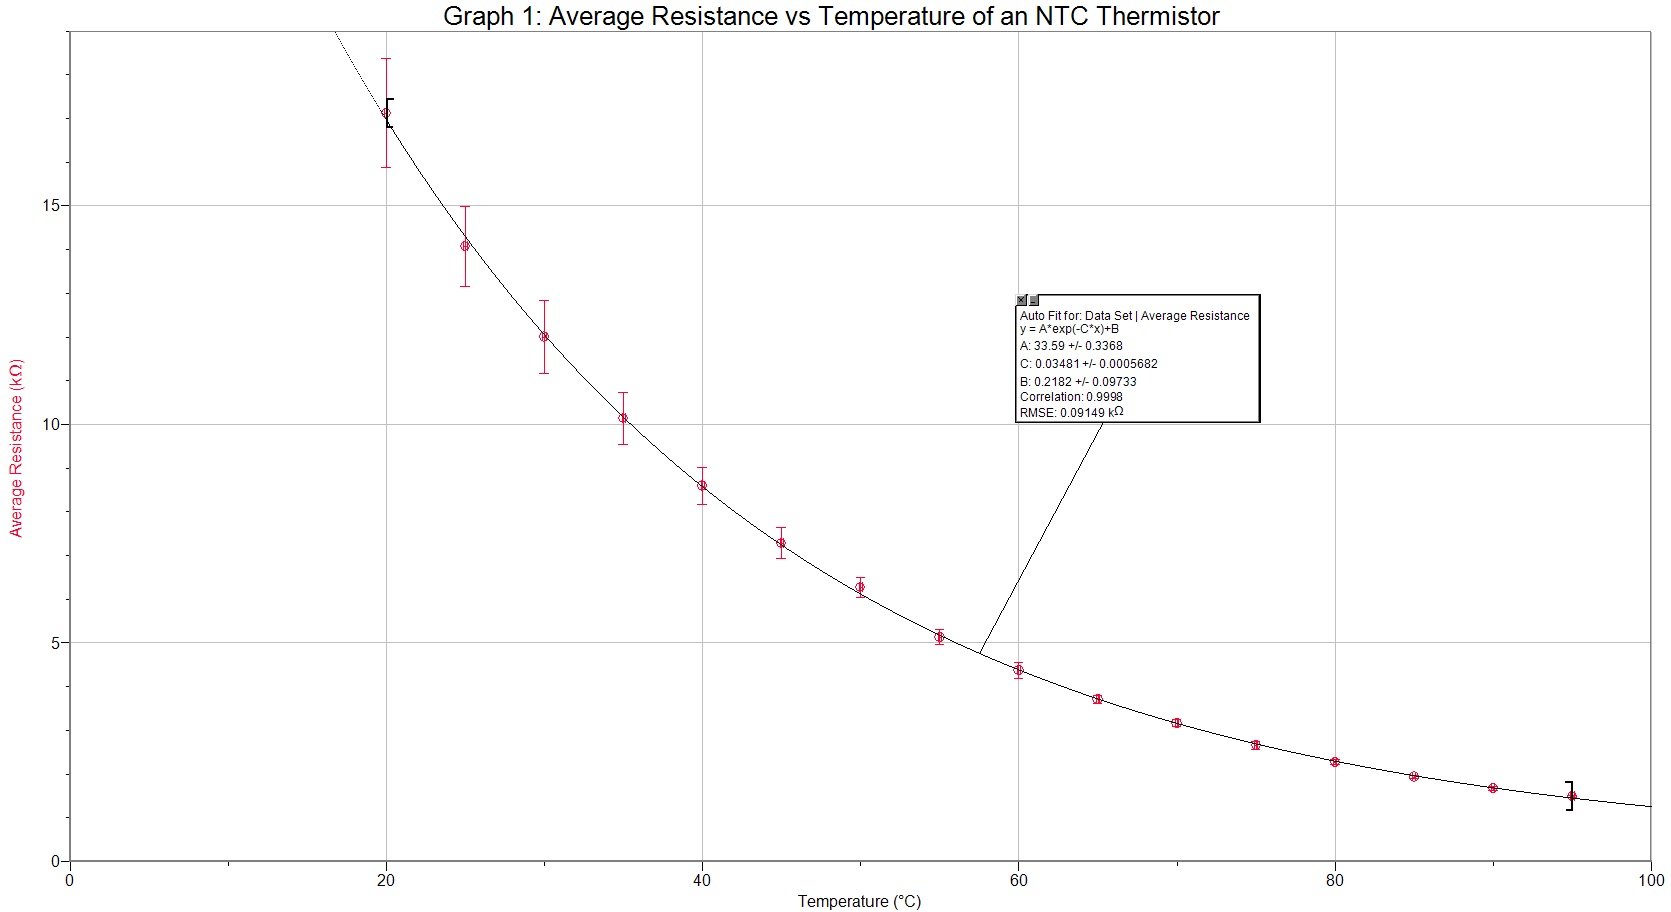
\includegraphics[width=120mm,height=\textheight,keepaspectratio]{images/before_linearization.png}
    \caption{Graph of Average Resistance vs Temperature}
    \label{fig:before_linearization}
\end{figure}

\subsection{Linearization: Beta Model}
Since there is a very strong correlation ($R^2=0.9998$) of the data to an exponential fit (Figure \ref{fig:before_linearization}), the data should be linearized to better perform and interpret the slope. This data can be linearized using the Beta Model for a Thermistor shown below \citep{amethermbetamodel}.
\[\beta=\frac{\ln{\frac{R_2}{R_1}}}{\frac{1}{T_2}-\frac{1}{T_1}}\]
\[\ln{R_{avg}}=\beta\frac{1}{T}+\ln{R_0}\]

Note that the temperature is in Kelvin. Therefore, the following formula must be applied.

\[T_K=T_C+273\;K\]

The uncertainties for $\ln{R_avg}$ and $\frac{1}{T}$ can be determined using the Law of Propagation of Uncertainty \citep{taylor_1982}.
\[\delta f(x,y,\dots)=\sqrt{\left(\frac{\partial f}{\partial x}\delta x \right)^2+ \left(\frac{\partial f}{\partial y}\delta y \right)^2+\dots}\]

Thus, for $\ln{R_{avg}}$:
\[\delta \ln{(R_{avg})}=\sqrt{\left(\frac{\partial \ln{R_{avg}}}{\partial R_{avg}}\delta R_{avg} \right)^2}=\frac{\delta R_{avg}}{R_{avg}}=\frac{1.25\;k\Omega}{17.12\;k\Omega}=0.07 \;\ln{k\Omega}\]

Note that units for the linearized resistance are in $\ln{k\Omega}$, since they have a different dimension than the $k\Omega$.

Similarly, for $\frac{1}{T}$:
\[\delta \frac{1}{T}=\sqrt{\left(\frac{\partial \frac{1}{T}}{\partial T}\delta T \right)^2}=\frac{\delta T}{T^2}=\frac{0.1 K}{(293.0 \; K)^2}=0.000001 \;\frac{1}{K}\]

\begin{longtable}{| >{\centering\arraybackslash}p{0.2\linewidth} | >{\centering\arraybackslash}p{0.25\linewidth} | >{\centering\arraybackslash}p{0.15\linewidth} | >{\centering\arraybackslash}p{0.25\linewidth} |}
\hline
    Reciprocal of Temperature (1/K) & Reciprocal of Temperature Uncertainty (1/K) & ln of Average Resistance ($ln{k\Omega}$) & ln of Average Resistance Uncertainty ($ln{k\Omega}$) \\ \hline
    0.003413 & 0.000001 & 2.84 & 0.07 \\ \hline
    0.003356 & 0.000001 & 2.64 & 0.07 \\ \hline
    0.003300 & 0.000001 & 2.48 & 0.07 \\ \hline
    0.003247 & 0.000001 & 2.32 & 0.06 \\ \hline
    0.003195 & 0.000001 & 2.15 & 0.05 \\ \hline
    0.003145 & 0.000001 & 1.98 & 0.05 \\ \hline
    0.003096 & 0.000001 & 1.84 & 0.04 \\ \hline
    0.003049 & 0.000001 & 1.64 & 0.03 \\ \hline
    0.003003 & 0.000001 & 1.47 & 0.04 \\ \hline
    0.002959 & 0.000001 & 1.31 & 0.03 \\ \hline
    0.002915 & 0.000001 & 1.15 & 0.03 \\ \hline
    0.002874 & 0.000001 & 0.97 & 0.03 \\ \hline
    0.002833 & 0.000001 & 0.82 & 0.03 \\ \hline
    0.002793 & 0.000001 & 0.66 & 0.02 \\ \hline
    0.002755 & 0.000001 & 0.51 & 0.02 \\ \hline
    0.002717 & 0.000001 & 0.40 & 0.01 \\ \hline
    \caption{Natural Log of Average Resistance vs Reciprocal of Temperature of an NTC Thermistor}
\end{longtable}

\begin{figure}[H]
    \centering
    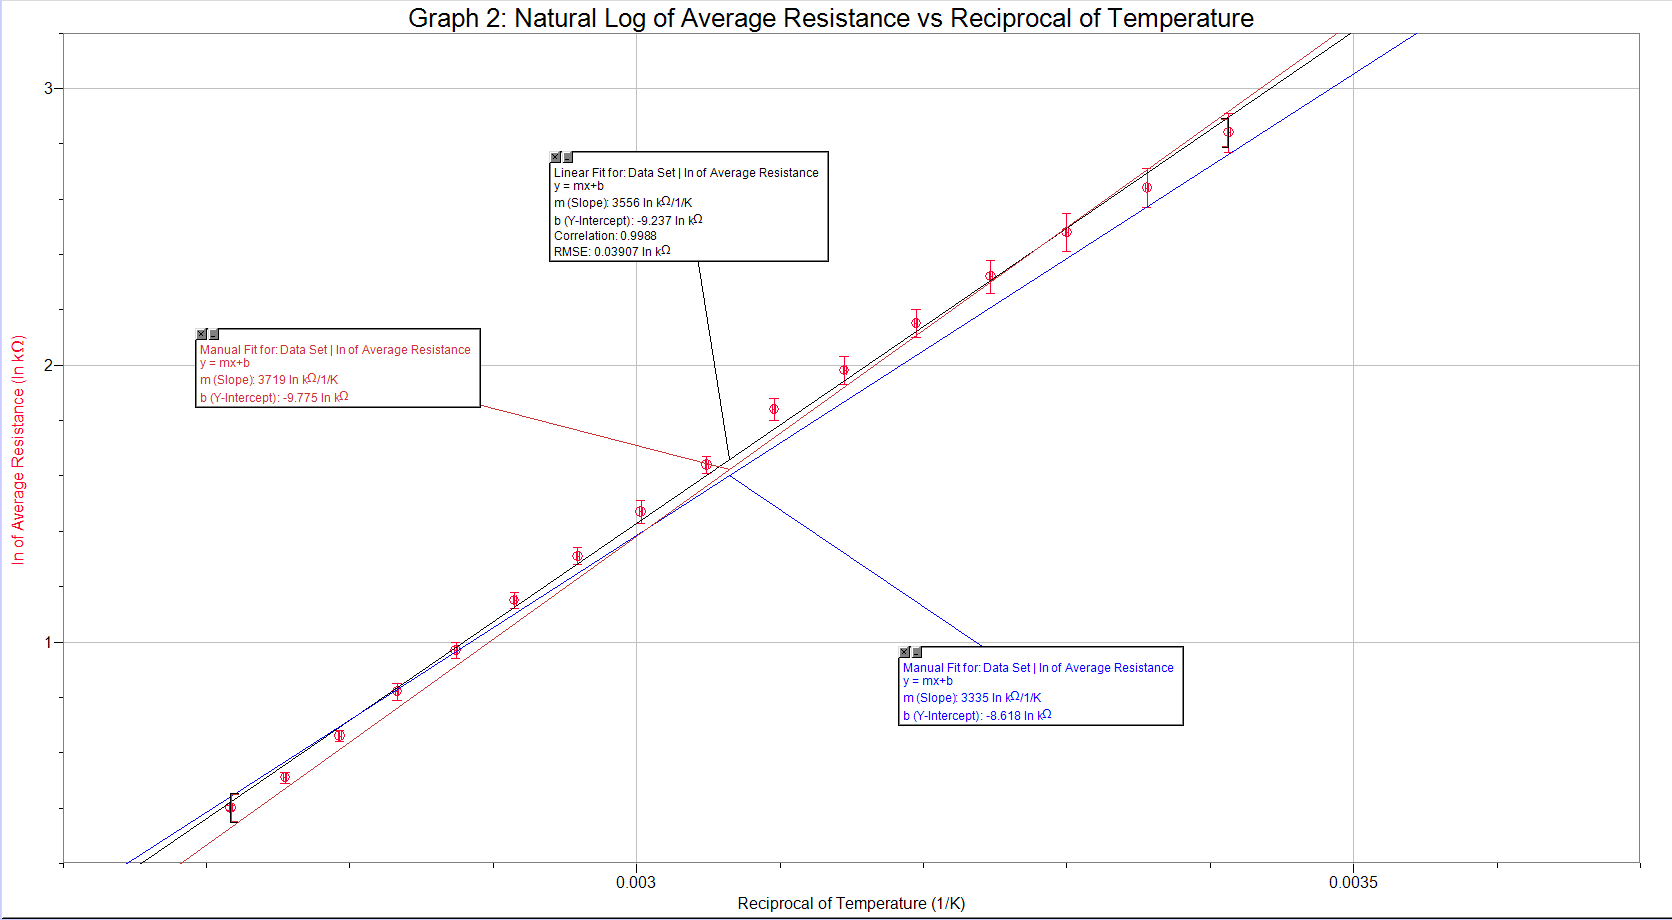
\includegraphics[width=120mm,height=\textheight,keepaspectratio]{images/after_linearization.png}
    \caption{Graph of Natural Log of Average Resistance vs Reciprocal of Temperature}
    \label{fig:after_linearization}
\end{figure}

\subsection{Percent Uncertainty and Percent Error of Slope}
A rough estimate of the percent uncertainty of the slope $\beta$ can be determined by utilizing the maximum and minimum slope lines.
\[\delta \beta = \frac{\beta_{max}-\beta_{min}}{2} = \frac{3719 K \ln{k\Omega}-3335 K \ln{k\Omega}}{2}=192 K \ln{k\Omega}\]
\[\frac{\delta \beta}{\beta}=\frac{192 K \ln{k\Omega}}{3556 K \ln{k\Omega}}=5.40 \%\]

The accepted value for the slope $\beta$ for this NTC Themistor is $3474 K \ln{k\Omega}$.
Therefore, to calculate the percent error, the following calculation can be performed.
\[Percent \; Error = \frac{|\beta_{actual} - \beta_{accepted}|}{\beta_{accepted}}=\frac{|3556 K \ln{k\Omega} - 3474 K \ln{k\Omega}|}{3474 K \ln{k\Omega}}=2.36\%\]


\subsection{Interpretation}
As seen in the Linearized Beta Model Graph (Figure \ref{fig:after_linearization}), the line of best fit indicates a positive linear relationship between $\ln{R}$ and $\frac{1}{T}$. This means as $\frac{1}{T}$ increases, $\ln{R}$ will increase proportionally. Furthermore, this linearization proves that there is a negative exponential relationship between $R$ and $T$.

There is a very strong correlation ($R^2=0.9988$) between the linear regression and the linearized data. The line of best fit passes through almost all points and uncertainty bars. The minimum and maximum slope lines are very similar to the regression line. All this affirms that the $R$ and $T$ for an NTC Thermistor follow a negative exponential relationship.

Finally, the slope $\beta$ of this graph represents the sensitivity of the thermistor's resistance to a change in temperature. A high $\beta$ indicates a more elastic relationship between resistance and temperature, and a low $\beta$ indicates a more more inelastic relationship.

\section{Conclusion}
Therefore, according to this experiment, there is a very strong correlation ($R^2=0.9988$) for a negative exponential relationship between the resistance and the temperature of an NTC Thermistor.
This matches my hypothesis for this experiment. Furthermore, the individual trial percent uncertainties were far below 5\%, which means that our measurement system is precise. However, some of the average percent uncertainties for the resistances at low temperatures were above 5\%, which means that the experiment had a bad procedure for these levels. Finally, since the uncertainty for the slope $\beta$ was less than 5\% and greater than the percent error for $\beta$, the final experiment results were precise and accurate.

\section{Sources for Error}
Error could have been introduced from 4 sources: measurement of temperature using the Vernier Temperature Probe, measurement of resistance using the Multimeter, data collection using video analysis, and the indirect heating of the thermistor using a water medium.

First, the measurement of temperature using the Vernier Temperature Probe contributes to random error since the device uncertainty for the probe is $\pm\;0.1^\circ C$. This random error from this source is negligible in this experiment. Next, the measurement of resistance using the Multimeter also contributes to random error since the device uncertainty for the device is $\pm\;0.01\;k\Omega$. This random error from this source is negligible at high temperatures, but at lower temperatures ($\le 35.0^\circ C$) the percent uncertainties exceeded 5\% indicating a significant random error. Then, since all temperature and resistance measurements were derived through video analysis, some random error was introduced. However, the accurate scrubbing on high frame rate and high-resolution videos utilized in the analysis significantly mitigated random error over collecting the data by eye. Therefore, the random error from this source is negligible in this experiment. Finally, since the thermistor was indirectly heated through a water medium, the temperature of the water could have been higher than that of the thermistor leading to systematic error. However, since the heating was put on the lowest setting, the temperature increased evenly and steadily, hence minimizing this error.

In conclusion, most sources of error were minimal throughout the experiment. However, the greater than 5\% percent uncertainties for resistance measurements at low temperatures due to random error were significant.

\section{Strengths}
One strength of this experiment is the use of video analysis to collect accurate temperature and resistance measurements. As the temperature steadily and evenly rose while being heated, video analysis was much more accurate than manually collecting the data by eye during the experiment. This also enabled me to take more frequent measurements, which helped me create more levels and hence data points for my regressions. Another strength of this experiment was the slow cooling procedure. After each trial, all equipment (beaker, temperature probe, and thermistor) was gradually cooled down back to room temperature. This ensured that the equipment did not experience a rapid temperature change, which could wear it down or damage it leading to varying results. Thus, in each trial, all equipment started in the same state as the previous trial. Finally, the slow heating utilized during the experiment was a major strength of this experiment. The slow heating ensured that the temperature rose steadily and evenly allowing for accurate and precise data collection through the video analysis. Furthermore, the slow heating mitigated systematic errors due to the differences in temperatures of the water, temperature probe, and thermistor.

\section{Weaknesses}
One weakness of this experiment is the loose connections between the circuit elements leading to variable results. Since alligator clips were utilized to connect the leads of the Multimeter to the NTC Thermistor, slightly loose values would cause significant variations in resistance readings. Furthermore, another weakness of this experiment is the NTC Thermistor utilized in this experiment. This thermistor had low accuracy at lower temperatures creating high random error, which led to the high average percent uncertainties for temperatures below $35.0^\circ C$. These were major experiment design flaws that need to be revised for future trials.

\section{Improvements}
There are multiple improvements that could be applied to this experiment to address its weaknesses. First, fewer connections in the circuit could be utilized to reduce the effect of loose connections. Specifically, the Multimeter could be directly attached to the NTC thermistor rather than via alligator clips. Second, an NTC thermistor with better accuracy at lower temperatures ($\le 35.0^\circ C$) could be used. This would reduce the high random error and hence the high average percent uncertainty for these temperatures. These improvements would greatly improve both the accuracy and precision of this experiment.

\section{Extensions}
There are multiple extensions to this experiment that might be worthy of future study. First, as mentioned in the Section \ref{section:introduction} \nameref{section:introduction}, this experiment could be extended to test the relationship between the resistance and temperature of a superconductor. Specifically, It would be interesting to see the change in this relationship prior to and after the critical temperature $T_c$ of a superconductive material such as YBCO. This experiment could be conducted in a similar fashion to this experiment, except, instead of using a range of temperatures above room temperature, liquid nitrogen could be used to achieve a range below and above the $T_c$ of a YBCO at 93 K \citep{butera1997dependence}.
Another experiment could explore other models to describe the relationship between the resistance and temperature of a thermistor. In industry, the Steinhart-Hart Model, an extension of the Beta Model used in this experiment, is used to describe this relationship. The following  is the equation for the Steinhart-Hart Model:
\[\frac{1}{T}=A+B\ln{R}+C[\ln{R}]^3\]
The procedure for the experiment would be similar to this experiment, but rather than using an exponential fit and the Beta Model to linearize my data, a cubic polynomial fit and the Steinhart-Hart Model would be utilized. This will improve the accuracy of the regression even more as the Beta Model simplifies the Steinhart-Hart Model by removing its cubic term \citep{rana2018fpga}.


\newpage
\bibliography{ref}
\bibliographystyle{apalike}

\end{document}
